\documentclass[11pt,a4paper,oneside]{scrartcl}
\usepackage[utf8]{inputenc}
\usepackage[english]{babel}
\usepackage{amsmath}
\usepackage{amsfonts}
\usepackage{amssymb}
\usepackage{graphicx}
\usepackage{lmodern}
\usepackage{url}
\usepackage{subfigure}

\usepackage{pgfplots}
\pgfplotsset{compat=newest}
\usepackage{tikz}



\usepackage[lmargin = 2cm,rmargin=2cm, tmargin = 2cm,bmargin=2cm]{geometry}

% Listings options
\usepackage{listings}
\usepackage{xcolor}
\definecolor{zebg}{rgb}{1,1,.8} %elfenbeinfarbig

\lstset{language=Matlab, numbers=left, numberstyle=\tiny, basicstyle=\footnotesize,showstringspaces=false,%
 numberblanklines=false, frame=single, backgroundcolor=\color{zebg},xleftmargin=0cm, linewidth=1.11\linewidth}



\author{Lars Schiller}
\title{Simulation of a satellite trajectory}

\begin{document}
\maketitle
\tableofcontents

\section{Introduction and task description}

Ziel des Wettbewerbs ist die numerische Simulation der ebenen Flugbahn eines Satelliten
um die Erde. Es sollen hierbei die Gravitationskräfte zwischen dem Satelliten, der Erde
und der Sonne beachtet werden, wobei die Gravitationskonstante 
$\gamma$ = 1 beträgt. Alle
weiteren Effekte dürfen vernachlässigt werden. The initial conditions are given with

\begin{tabular}{c|*{12}c|*{3}c|c}
&$r_{1x}$ & $r_{1y}$ & $r_{2x}$ & $r_{2y}$ & $r_{3x}$ & $r_{3y}$ & $\dot{r}_{1x}$ & $\dot{r}_{1y}$ & $\dot{r}_{2x}$ & $\dot{r}_{2y}$ & $\dot{r}_{3x}$ & $\dot{r}_{3y}$ &$m_1$&$m_2$&$m_3$ & $\gamma$\\ \hline
value: &  0 & 0 & 20 & 0 & 20 & -2 & -.02 & -.22 & 0 & 2 & 2.1 & 2.1 & 100 & 10 & 1 & 1 \\
\end{tabular}.



\section{Mathematical model of the task}
In the following the sun will be subscripted by 1, the earth by 2 and the satellite by 3. Furthermore vectors will be written as bold symbols, like $\boldsymbol{r}_1$ as the position vector of the sun.


\begin{figure}[ht]
\begin{center}
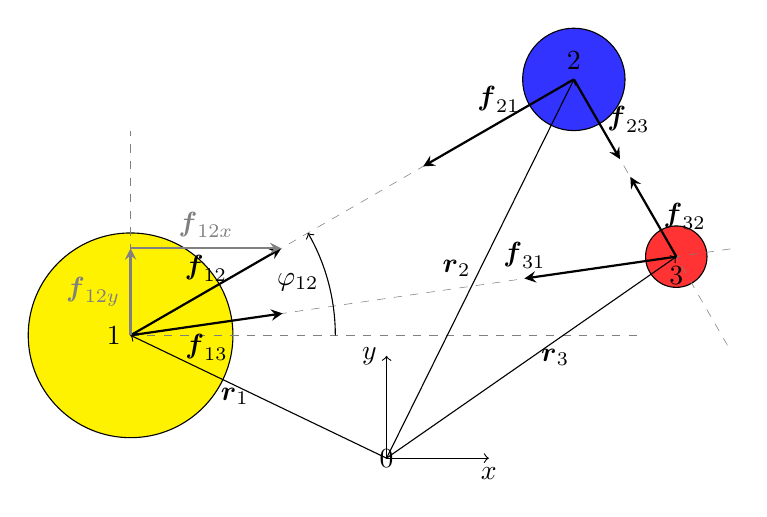
\begin{tikzpicture}[scale=1.3]
%% Coordsys
\draw[->] (2.5,-1.2)coordinate(0)node{0}--++(1,0)node[below]{$x$};
\draw[->] (0)--++(0,1)node[left]{$y$};
%% Objects
\draw[fill=yellow] (0,0)circle(1)node[left]{1}coordinate(1);
\draw[fill=blue!80] (30:5)circle(.5)node[above]{2}coordinate(2);
\draw[fill=red!80] (2)++(-60:2)circle(.3)node[below]{3}coordinate(3);
%% Help Lines
\draw[help lines,dashed] (1)--++(5,0);
\draw[help lines,dashed] (1)--++(0,2);
\draw[help lines,dashed] (1)--++(30:5);
\draw[help lines,dashed] (1)--++(8.2:6);
\draw[help lines,dashed] (2)--++(-60:3);
%% Vecs
\draw[->] (0)--(1)node[midway,left]{$\boldsymbol{r}_1$};
\draw[->] (0)--(2)node[midway,left]{$\boldsymbol{r}_2$};
\draw[->] (0)--(3)node[midway,right]{$\boldsymbol{r}_3$};
%% Forces
\draw[thick,-stealth] (1)--++(30:1.7)node[above,midway]{$\boldsymbol{f}_{12}$};
\draw[thick,-stealth] (1)--++(8.2:1.5)node[below,midway]{$\boldsymbol{f}_{13}$};
\draw[thick,-stealth] (2)--++(210:1.7)node[above,midway]{$\boldsymbol{f}_{21}$};
\draw[thick,-stealth] (2)--++(-60:.9)node[right,midway]{$\boldsymbol{f}_{23}$};
\draw[thick,-stealth] (3)--++(180-60:.9)node[right,midway]{$\boldsymbol{f}_{32}$};
\draw[thick,-stealth] (3)--++(180+8.2:1.5)node[above]{$\boldsymbol{f}_{31}$};
\draw[thick,-stealth,gray] (1)--++(90:.5*1.7)node[midway,left]{$\boldsymbol{f}_{12y}$};
\pgfmathsetmacro{\l}{sqrt(3)/2*1.7}
\draw[thick,-stealth,gray] (1)++(90:.5*1.7)--++(0:\l)node[midway,above]{$\boldsymbol{f}_{12x}$};
\draw[->] (1)++(0:2)arc(0:30:2);
\path (1)++(15:2)node[left]{$\varphi_{12}$};
\end{tikzpicture}
\end{center}
\caption{Resultant Forces on the objects}
\label{fig:forces}
\end{figure}


From \textit{Newtons} Gravity Law it is known\footnote{\url{http://en.wikipedia.org/wiki/Newton's_law_of_universal_gravitation}} that mass afflicted bodies generate forces to each other with the following rule:
\begin{equation}
F = \gamma \frac{m_1m_2}{|\boldsymbol{r}|^2}.
\label{eq:newtonsgrav}
\end{equation}
The problem we have two solve consist of three mass points with two degrees of freedom respectively. The resultant forces between these points can be described with respect to equation~\ref{eq:newtonsgrav} by:
\begin{equation}
\boldsymbol{f}_{ij} = \underbrace{\gamma \frac{m_im_j}{|\boldsymbol{r}_j-\boldsymbol{r}_i|^2}}_{\textnormal{magnitude}} ~ \underbrace{\frac{\boldsymbol{r_j}-\boldsymbol{r}_i}{|\boldsymbol{r_j}-\boldsymbol{r}_i|}}_{\textnormal{direction}} = \gamma \frac{m_im_j}{|\boldsymbol{r}_j-\boldsymbol{r}_i|^3} \left( \boldsymbol{r_j}-\boldsymbol{r}_i \right),
\label{eq:forces}
\end{equation}
where $i,j$ are the indices of the mass points. The force $\boldsymbol{f}_{ij}$ acts on the point $i$ and is generated by the presence of point $j$. To obtain the $x$-part of the force one can scalar multiply $\boldsymbol{f}_{ij}$ with the unit vector in $x$-direction, and accordingly with $y$:
\begin{equation}
{f}_{ijx} = \boldsymbol{f}_{ij}^T\boldsymbol{e}_{x} ,\qquad {f}_{ijy} = \boldsymbol{f}_{ij}^T\boldsymbol{e}_{y} 
\end{equation}
Figure~\ref{fig:forces} illustrates these forces.
In aim to obtain a differential equation to simulate the given task one can use \textit{Newtons} Second Law:
\begin{equation}
m\ddot{r} = \sum\limits_n f_n.
\label{eq:newtons2nd}
\end{equation}
Since this is a differential equation of order 2, we can use the well known trick and reformulate equation~\ref{eq:newtons2nd} in:
\begin{equation}
\left[
\begin{matrix}
1 & 0 \\
0 & \boldsymbol{M} 
\end{matrix}
\right]
\left[
\begin{matrix}
\dot{\boldsymbol{r}} \\
\ddot{\boldsymbol{r}}
\end{matrix}
\right]
= 
\left[
\begin{matrix}
0 & 1 \\
\boldsymbol{f}(\boldsymbol{r}) & 0 
\end{matrix}
\right]
\left[
\begin{matrix}
{\boldsymbol{r}} \\
\dot{\boldsymbol{r}}
\end{matrix}
\right]
\label{eq:soe},
\end{equation}
where $\boldsymbol{M}$ is the mass matrix and  $\boldsymbol{f}(\boldsymbol{r})$ denotes a function which depends on the actual position of the objects. By defining the state vector $\boldsymbol{x}$ as:
$$
\boldsymbol{x} = \left[ r_{1x} ~~ r_{1y} ~~ r_{2x} ~~ r_{2y} ~~ r_{3x} ~~ r_{3y} ~~ \dot{r}_{1x} ~~ \dot{r}_{1y} ~~ \dot{r}_{2x}  ~~ \dot{r}_{2y} ~~ \dot{r}_{3x} ~~ \dot{r}_{3y} \right]^T
$$
equation ~\ref{eq:soe} can be written as
\begin{equation}
\dot{\boldsymbol{x}}
=
\left[
\begin{matrix}
\boldsymbol{x}(7:12) \\
\frac{1}{m_1} \left( f_{12x} + f_{13x} \right) \\
\frac{1}{m_1} \left( f_{12y} + f_{13y} \right) \\
\frac{1}{m_2} \left( f_{21x} + f_{23x} \right) \\
\frac{1}{m_2} \left( f_{21y} + f_{23y} \right) \\
\frac{1}{m_3} \left( f_{31x} + f_{32x} \right) \\
\frac{1}{m_3} \left( f_{31y} + f_{32y} \right) \\
\end{matrix}
\right]
\label{eq:ode}
\end{equation}
This is a non-linear ordinary system of differential equations, which can be solved with the known methods, like the advanced \textit{Euler}-Method.

\section{Description and evaluation of the results}

The results shown in figure~\ref{fig:sol_1e-3} are obtained by the \texttt{Matlab} implemented solvers \texttt{ode45},\texttt{ode113}, \texttt{ode15s} and the self-written solver \texttt{euler.m} with a relative tolerance of \texttt{1e-3}. The results shown in figure~\ref{fig:sol_1e-6} are obtained by the same solvers, but with a relative tolerance of \texttt{1e-6}, except the \textit{Euler}-method, which has a relative tolerance of \texttt{1e-4}, due to the massive computational effort.

It's easy to see, that the results shown in figure~\ref{fig:sol_1e-3} are inconsistent. For example in figure~\ref{fig:sol_1e-3}(a) the satellite is going to crash with the earth. This is reasoned by the fact that for the given problem a high accuracy is necessary. By increasing the relative tolerance the results of every method become similar. In table~\ref{tab:eva} the number of needed supporting points of every solving method are listed. For the needed high accuracy \texttt{ode113} get along with least supporting points and therefore with least computational effort.


\section{Interpretation of the results}
Since the the results of every solving method are nearly the same for a tight relative tolerance, its reasonable to trust in these. 
Therefore with the assumptions we have done and with the given initial conditions, the trajectory of the satellite will stable. But with a little phase shift of the satellite per rotation around the sun by the earth. By accepting this, a later control will not be  necessary. 


\begin{figure}
\begin{centering}
\subfigure[\texttt{ode45}]{
\includegraphics[width=.235\textwidth]{sol_1e-3/sol_ode45_100_1e-3.pdf}}
\subfigure[\texttt{ode113}]{
\includegraphics[width=.235\textwidth]{sol_1e-3/sol_ode113_100_1e-3.pdf}}
\subfigure[\texttt{ode15s}]{
\includegraphics[width=.235\textwidth]{sol_1e-3/sol_ode15s_100_1e-3.pdf}}
\subfigure[\textit{Euler}]{
\includegraphics[width=.235\textwidth]{sol_1e-3/sol_odee_100_1e-3.pdf}}
\end{centering}
\caption{Results of the Simulation obtained by several numerical solvers with \texttt{RelTol = 1e-3}}
\label{fig:sol_1e-3}
\end{figure}
\begin{figure}
\begin{centering}
\subfigure[\texttt{ode45}]{
\includegraphics[width=.235\textwidth]{sol_1e-6/sol_ode45_100_1e-6.pdf}}
\subfigure[\texttt{ode113}]{
\includegraphics[width=.235\textwidth]{sol_1e-6/sol_ode113_100_1e-6.pdf}}
\subfigure[\texttt{ode15s}]{
\includegraphics[width=.235\textwidth]{sol_1e-6/sol_ode15s_100_1e-6.pdf}}
\subfigure[\textit{Euler}]{
\includegraphics[width=.235\textwidth]{sol_1e-6/sol_odee_100_1e-6.pdf}}
\end{centering}
\caption{Results of the Simulation obtained by several numerical solvers with \texttt{RelTol = 1e-6}}
\label{fig:sol_1e-6}
\end{figure}
\begin{table}
\begin{center}
\begin{tabular}{c|cccc}
 & \texttt{ode45} & \texttt{ode113} & \texttt{ode15s} & Advanced \textit{Euler} \\ 
\hline 
supporting points (\texttt{RelTol = 1e-3}) & 1309 & 688 & 866 & 6410 \\ 
supporting points (\texttt{RelTol = 1e-6}) & 2881 & 1249 & 2180 & - \\ 
supporting points (\texttt{RelTol = 1e-4}) & - & - & - & 20292 \\ 
\end{tabular} 
\end{center}
\caption{Evaluation of the results}
\label{tab:eva}
\end{table}



\end{document} 